\documentclass[article]{jss}

%% -- LaTeX packages and custom commands ---------------------------------------

%% recommended packages
\usepackage{orcidlink,thumbpdf,lmodern}

%% another package (only for this demo article)
\usepackage{framed}

%% new custom commands
\newcommand{\class}[1]{`\code{#1}'}
\newcommand{\fct}[1]{\code{#1()}}

%% For Sweave-based articles about R packages:
%% need no \usepackage{Sweave}



%% -- Article metainformation (author, title, ...) -----------------------------

%% - \author{} with primary affiliation (and optionally ORCID link)
%% - \Plainauthor{} without affiliations
%% - Separate authors by \And or \AND (in \author) or by comma (in \Plainauthor).
%% - \AND starts a new line, \And does not.
\author{Paul Kruse~\orcidlink{0000-0003-0918-3766}\\US Environmental Protection Agency
   \And Caroline Ring~\orcidlink{0000-0002-0463-1251}\\US Environmental Protection Agency}
\Plainauthor{Paul Kruse, Caroline Ring}

%% - \title{} in title case
%% - \Plaintitle{} without LaTeX markup (if any)
%% - \Shorttitle{} with LaTeX markup (if any), used as running title
\title{treecompareR: }
\Plaintitle{treecompareR: }
\Shorttitle{\pkg{treecompareR}:}

%% - \Abstract{} almost as usual
\Abstract{
  This paper presents the \pkg{treecompareR} package for \proglang{R}, which provides tools for reproducible visualizations of data through the use of taxonomies. The package builds on developments from \pkg{ggplot2} and \pkg{ggtree} to provide visualizations tailored for use with taxonomic classification data. It also provides a pipeline for gathering chemical classification data using \pkg{classyfireR}. Additionally, it provides tools that leverage developments in network analysis to compare data sets. While designed specifically for chemical classification objectives using ClassyFire(\url{http://classyfire.wishartlab.com/}), \pkg{treecompareR} provides tools for use with more general taxonomies.
}

%% - \Keywords{} with LaTeX markup, at least one required
%% - \Plainkeywords{} without LaTeX markup (if necessary)
%% - Should be comma-separated and in sentence case.
\Keywords{JSS, style guide, comma-separated, not capitalized, \proglang{R}}
\Plainkeywords{JSS, style guide, comma-separated, not capitalized, R}

%% - \Address{} of at least one author
%% - May contain multiple affiliations for each author
%%   (in extra lines, separated by \emph{and}\\).
%% - May contain multiple authors for the same affiliation
%%   (in the same first line, separated by comma).
\Address{
  Paul Kruse\\
  Center for Computational Toxicology and Exposure\\
  United States Environmental Protection Agency\\
  109 TW Alexander Dr, Durham, NC 27709, United States of America\\
  E-mail: \email{kruse.paul@epa.gov}
}

\begin{document}


%% -- Introduction -------------------------------------------------------------

%% - In principle "as usual".
%% - But should typically have some discussion of both _software_ and _methods_.
%% - Use \proglang{}, \pkg{}, and \code{} markup throughout the manuscript.
%% - If such markup is in (sub)section titles, a plain text version has to be
%%   added as well.
%% - All software mentioned should be properly \cite-d.
%% - All abbreviations should be introduced.
%% - Unless the expansions of abbreviations are proper names (like "Journal
%%   of Statistical Software" above) they should be in sentence case (like
%%   "generalized linear models" below).

\section[Introduction} \label{sec:intro}

Classification of objects has been a source of much development of organizational structures across various fields of science. Organizing objects into a coherent structure helps one to understand how these objects relate to each other and can lead to the discovery of connections between various sets of objects. How one organizes the objects may depend on underlying attributes that the objects possess.

Ontologies provide a framework for comparing objects through a variety of different relation types. These relation types create a network structure that can be studied using graph theory techniques. One of the more actively developed ontologies in recent science is the Gene Ontology, which aims to develop a computation model of biological systems. The ontology considers the three domains defined as molecular function, cellular component, and biological process with relationships between terms within each of these domains and between the three domains as well. Using these domains, the ontology describes genes and how they relate to various areas of interest in contemporary biological research.

Within the universe of ontologies sits the set of organizing structures known as taxonomies. Restricting the attention to taxonomies, one can focus specifically on the “is a” relation, e.g. “a dog (canis familiaris) is a canis” and study how objects relate to one another under this specific relationship scheme. One well known example of this organizational structure in use is the Linnaean system for classifying life, sometimes referred to as the “tree of life”. As a taxonomy, the organizational structure is given by a tree, which consequently lends itself to analysis using tree-based techniques from graph theory.

In 2016, the ClassyFire (http://classyfire.wishartlab.com/) tool was introduced, in the work of \cite{djoumbou2016classyfire}. This work presented a chemical ontology, ChemOnt, consisting of 4825 classification labels. These labels are organized in a taxonomy structure with pairs of distinct labels either satisfying a simple "is a" relation or not. The ClassyFire tool takes in chemical identifiers such as InChIKey or SMILES strings and provides a classification of the chemical within the taxonomy. In this manner, one can examine a data set consisting of chemical data from the viewpoint of where the chemicals lie within the ChemOnt taxonomy structure.

In the study of cheminformatics, machine-learning models such as Quantitative structure-activity relationship (QSARs) are constructed to link physical and structural properties with biological interactions. For these models to produce accurate and reliable predictions, an analysis of the training data and targeted use data is essential. This consideration of the domain of applicability of the model is important for determining when the trained model’s predictions can be considered reliable given an input chemical. In many cases, this analysis can be carried out using model descriptors, for example by using structural descriptors of the molecules used for training the model. However, while descriptors may accurately describe the domain of applicability, they often can be hard to interpret and they do not necessarily lend themselves that well to visualization.

Understanding and overcoming these issues in one’s ability to interpret the data are especially important when comparing pairs of data sets, such as training and test sets or training and prediction sets. While it may be feasible to examine how each individual data set is characterized by model descriptors, how they overlap requires additional consideration. Is the overlap broad or does it focus on specific areas? Are there gaps between the training data and prediction data that may reduce the confidence users have in model predictions? Answering these and other questions addresses concerns of model applicability to data sets in general and how the model can be improved regarding gaps in training data compared to prediction or test data.

One approach to addressing these naturally arising concerns is through visualizations that can increase the user’s ability to interpret the data sets. Since the ClassyFire ChemOnt ontology is organized in a taxonomy structure, one can leverage the tree structure not only for quantitative analysis but also through the use of tree visualizations. These visualizations can reveal the extent to which there are overlaps within the data and the degree of such overlaps. The diagrams also show very clearly when there are gaps between the data sets and broad coverage, or lack thereof, within the chemical universe as it is represented by ChemOnt.

However, such visualizations are limited in terms of what is currently available. One may use the \pkg{ggplot2} \proglang{R} package to visualize statistics based on the taxonomic information corresponding to classifications of a data set \cite{ggplot22016} . But \pkg{ggplot2} is a very broad package and not designed for handling chemical classification data in particular. Since the ChemOnt taxonomy is given by a tree structure, one can use tree visualization packages such as \pkg{ggtree} to visualize this structure \cite{yu2017ggtree}. However, the \pkg{ggtree} package was designed with phylogenetic trees in mind, which are generally presented as rooted binary trees (possibly with additional data). The ChemOnt ontology is neither a binary tree nor does it carry additional explicit data, so \pkg{ggtree} is again a very broad approach to this.  The package \pkg{treecompareR} leverages several \proglang{R} packages designed for tree manipulation and exploration, including \pkg{phytools} \cite{phytools2024revell}, \pkg{phangorn} \cite{phangorn2011schliep, phangorn2017schliep}, \pkg{Ape} \cite{ape2019paradis}, \pkg{Treeio} \cite{treeio2020Wang}. It also combines tree visualizations with heatmaps, in particular using the package \pkg{ComplexHeatmap} \cite{complexheatmap2016gu}.

We present the package \pkg{treecompareR} as a solution to the specific needs of creating a pipeline to classify chemicals in a data set, visualize the chemical space they represent, and compare the data sets from the point of view of chemical space. We introduce the package through a case study analyzing two specific data sets. We characterize two data sets, named \code{BIOSOLIDS} and \code{USGSWATER}, that were collected from the CompTox Chemical Dashboard \cite{williams2017comptox}. The \code{BIOSOLIDS} data describe chemicals detected in biosolids, as reported by three national sewage sludge surveys and eight biennial reviews, while the \code{USGSWATER} data describe chemicals found in water by the USGS.

We are interested in studying these two data sets together for a variety of reasons. The presence of chemicals detected in water is important information to consider when determining risk assessment for human and ecological health. Not only does this indicate what chemicals human activity contributes to water, but also what to expect to be present in water that is used in commercial, industrial, and residential settings. Chemicals detected in biosolids indicate both the chemicals that are already present in water in before being used, and the chemicals that human activity contributes to water and persists through the treatment process of waste water. By examining these two sets, we can get a better idea of which chemicals are introduced directly through human activity and use, and which chemicals are already in the background water as well as those that may be successfully removed from the water and captured within the biosolid.

\section{ClassyFire} \label{sec:class}

In this paper, we use the \code{chemical\_list\_BIOSOLIDS\_2022\_05\_10} and \code{chemical\_list\_USGSWATER\_2022\_05\_17} data sets, which are available for download from the US Environmental Protection Agency's Comptox Chemicals Dashboard \url{https://comptox.epa.gov/dashboard/chemical-lists}. Note, the names of these data sets as listed on the CompTox Dashboard Chemical List are \code{BIOSOLIDS2021} and \code{USGSWATER}, respectively.

These data sets include a list of chemicals, relevant identifiers such as \code{DTXSID}, \code{InChIKey}, \code{SMILES}, physico-chemical property data such as \code{MOLECULAR\_FORMULA}, \code{AVERAGE\_MASS}, \code{MONOISOTOPIC\_MASS}, and publication and quality data such as \code{PUBCHEM\_DATA\_SOURCES} and \code{QC\_Level}.

Before we start comparing these data sets, we must provide each chemical in each data set classification data from ClassyFire. To do this, we use the classification pipeline in \pkg{treecompareR}, construct a tree that encodes the taxonomy used in this classification scheme, and use this tree for data analysis and to create visualizations.

To achieve these aims, we use the ClassyFire tool found at \url{http://classyfire.wishartlab.com/}. ClassyFire uses the ChemOnt ontology, consisting of 4825 labels over 11 levels of classification, to classify chemicals. The ontology is given a taxonomic structure, that of a tree, with each label given a unique parent label and potentially having several children labels. This relationship data between labels can be found at the ChemOnt Taxnodes page \url{http://classyfire.wishartlab.com/tax_nodes.json} in JSON format. To construct a tree that encodes this structure, we must first download this data or use the file \code{chemont_parent_child.rda} from \pkg{treecompareR} with column names \code{Name}, \code{ID}, \code{Parent_ID}. With this data in hand, we construct the tree as a \code{phylo} object as follows.


%
\begin{Schunk}
\begin{Sinput}
R> chemont_taxonomy <- generate_taxonomy_tree(tax_nodes = chemont_df)
R> str(chemont_taxonomy[[1]], width = 60)
\end{Sinput}
\begin{Soutput}
 num [1:4824, 1:2] 3613 3614 3615 3615 3615 ...
\end{Soutput}
\begin{Sinput}
R> str(chemont_taxonomy[[2]], width = 60)
\end{Sinput}
\begin{Soutput}
 int 1213
\end{Soutput}
\begin{Sinput}
R> str(chemont_taxonomy, width = 60)
\end{Sinput}
\begin{Soutput}
List of 5
 $ edge       : num [1:4824, 1:2] 3613 3614 3615 3615 3615 ...
 $ Nnode      : int 1213
 $ tip.label  : chr [1:3612] "Thiepanes" "Benzoxazolines" "Polychlorinated dibenzofurans" "Polybrominated dibenzofurans" ...
 $ edge.length: num [1:4824] 9.09 11.36 79.55 79.55 19.89 ...
 $ node.label : chr [1:1213] "Chemical entities" "Organic compounds" "Organoheterocyclic compounds" "Benzofurans" ...
 - attr(*, "class")= chr "phylo"
 - attr(*, "order")= chr "cladewise"
\end{Soutput}
\end{Schunk}
%

The output of the \fct{generate\_taxonomy} function is a list of two objects, the \code{phlyo} object representing the tree, and a data frame used in creating the \code{phylo} object. Observe the structure of these in the code chunk above.

The \code{phylo} object itself is a list, describing the edges of the tree, the number of internal nodes, the tip labels and internal node labels, and a set of edge lengths generated in the construction of the tree. One thing to note is that the edge lengths are artificial and are only used to speed up the creation of the tree, but do not represent any actual data corresponding to the tree. However, we retain the edge lengths as they are useful in creating visualizations.

To construct a tree for other taxonomies, one can enter in a path to a JSON file or an enter in a data frame. The JSON file must have three columns, the first the name of the label \code{Name}, the second its identifier \code{ID}, and the third the parent identifier \code{Parent\_ID}. For the root, the parent ID should be \code{NA}. If the data is in the form of a data frame, it must be organized in the same way the JSON file is, with column names given by the same column names in the same order.

Next, we use the ClassyFire tool to provide classifications for the chemicals in our data sets. To simplify this process, \pkg{treecompareR} has a data pipeline that allows for programmatic acquisition of this data. It leverages the package \pkg{classyfireR} \url{https://github.com/aberHRML/classyfireR} for accessing the ClassyFire API. For chemical missing certain identifying data such as InChIKey or SMILES string data, we can use functions from the \proglang{R} package \pkg{ctxR} . We demonstrate how to use these below.

%
\begin{Schunk}
\begin{Sinput}
R> CASRN <- c('117964-21-3', '11006-76-1')
R> chemical_search <- ctxR::chemical_equal_batch(word_list = CASRN)
R> chemical_ids <- ctxR::get_chemical_details_batch(DTXSID = chemical_search$dtxsid)
R> data.table::setnames(x = chemical_ids, old = 'inchikey', new = 'INCHIKEY')
R> chemicals_class <- classify_datatable(chemical_ids[, .(INCHIKEY, dtxsid, casrn)])
R> str(chemicals_class)
\end{Sinput}
\begin{Soutput}
Classes 'data.table' and 'data.frame':	2 obs. of  17 variables:
 $ INCHIKEY  : chr  NA "AAFUUKPTSPVXJH-UHFFFAOYSA-N"
 $ dtxsid    : chr  "DTXSID40880080" "DTXSID9074775"
 $ casrn     : chr  "11006-76-1" "117964-21-3"
 $ smiles    : chr  NA "BrC1=CC(Br)=C(Br)C(Br)=C1OC1=C(Br)C(Br)=C(Br)C=C1Br"
 $ inchikey  : chr  NA "InChIKey=AAFUUKPTSPVXJH-UHFFFAOYSA-N"
 $ report    : chr  NA "ClassyFire returned a classification"
 $ kingdom   : chr  NA "Organic compounds"
 $ superclass: chr  NA "Benzenoids"
 $ class     : chr  NA "Benzene and substituted derivatives"
 $ subclass  : chr  NA "Diphenylethers"
 $ level5    : chr  NA "Bromodiphenyl ethers"
 $ level6    : chr  NA NA
 $ level7    : chr  NA NA
 $ level8    : chr  NA NA
 $ level9    : chr  NA NA
 $ level10   : chr  NA NA
 $ level11   : chr  NA NA
 - attr(*, ".internal.selfref")=<externalptr> 
 - attr(*, "sorted")= chr "INCHIKEY"
\end{Soutput}
\end{Schunk}
%

In this example, we input into the \fct{ctxR::chemical\_equal\_batch} function the list of CASRN strings. This searches and returns chemicals that match these values exactly. Next, the function \fct{ctxR::get\_chemical\_details\_batch} uses the \code{dtxsid} column values to retrieve the chemical details for these. Finally, we input as a \code{data.table} with columns \code{INCHIKEY},  \code{dtxsid}, and \code{casrn} into the function \fct{classify\_datatable}, which hits the ClassyFire API and attaches the retrieved information to the input data, as displayed. Note that the \code{CASRN} with value '117964-21-3' has both an \code{inchikey} and \code{smiles} value while the \code{CASRN} with value '11006-76-1' has neither piece of information. The ClassyFire data is available for the first chemical, but not the second.

We use the classified datasets \code{biosolids\_classified} and \code{usgswater\_classified} in several examples to follow.

If we examine the \code{usgswater\_classified} data as follows, we get the contents of
%
\begin{Schunk}
\begin{Sinput}
R> usgswater_classified[1:5, c('CASRN', 'kingdom', 'superclass', 'class', 'subclass')]
\end{Sinput}
\end{Schunk}
%

\begin{table}[t!]
\scriptsize
\centering
\begin{tabular}{llllp{2cm}}
\hline

CASRN &	kingdom &	superclass & class & subclass\\
\hline
7287-19-6 & Organic compounds	& Organoheterocyclic compounds &	Triazines	& 1,3,5-triazines	 \\
1031-07-8 &	Organic compounds &	Organic acids and derivatives &	Organic sulfuric acids and derivatives &	Sulfuric acid esters  \\
120868-66-8	& Organic compounds &	Organoheterocyclic compounds &	Pyridines and derivatives &	Halopyridines	\\
137-42-8	& Organic compounds	& Organic salts	& Organic metal salts	& Organic alkali metal salts	\\
82-86-0	& Organic compounds & Benzenoids	& Naphthalenes &	NA	\\
\hline

\end{tabular}
\caption{\label{tab:usgs-head} Overview of data contained in the \code{usgswater\_classified} classifications.}
\end{table}


Observe in the fifth row, the subclass label is given by NA. This means that the most specific classification label for this chemical is \code{Naphthalenes} at the \code{class} level. The chemicals in the previous rows have labels at least down to the \code{subclass} level, and potentially further, though this table is too small to illustrate the maximum classification depth for all of them (the chemical in the fourth row terminates at the \code{subclass} level while the three chemicals above it terminate at \code{level5}, the next level below).

To gain an understanding of these data sets and the chemical classifications they represent, we first look at the number of labels each data set represents, broken down through taxonomic level. The function \fct{label\_bars} takes in a single \pkg{data.table} or a (possibly named) list of \pkg{data.tables} and constructs histograms of label numbers faceted by data set and by taxonomic level.

%
\begin{Schunk}
\begin{Sinput}
R> data_list <- list(biosolids_classified,
+                    usgswater_classified)
R> names(data_list) <- c('Biosolids', 'USGS Water')
R> label_bars(data_list)
\end{Sinput}
\end{Schunk}
%

\begin{figure}[t!]
\centering
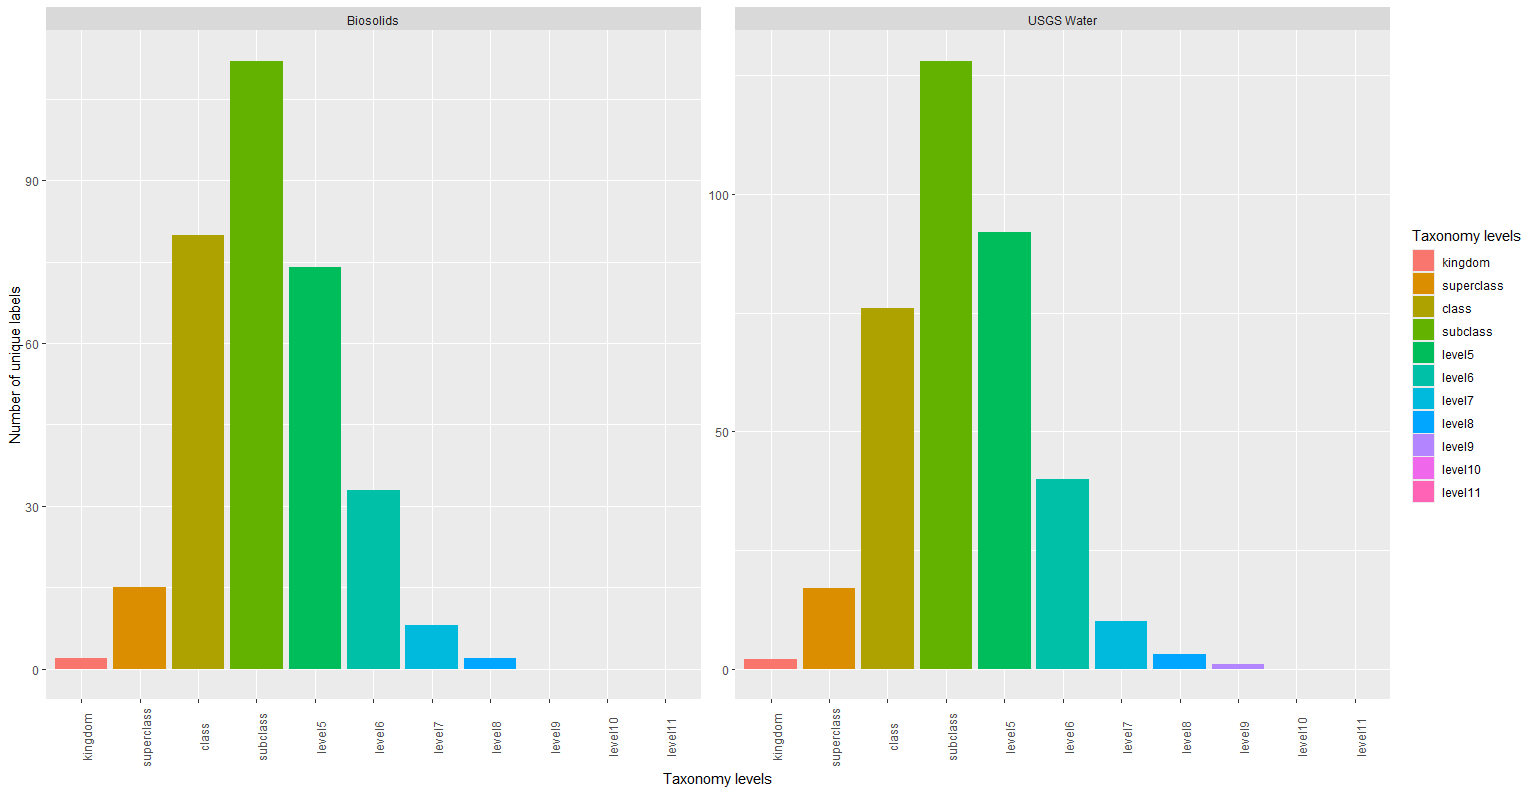
\includegraphics{label-bars_1}
\caption{\label{fig:lab-bars-1} This figure displays the counts of unique labels broken down by each classification level and faceted by dataset.}
\end{figure}

\begin{figure}[t!]
\centering
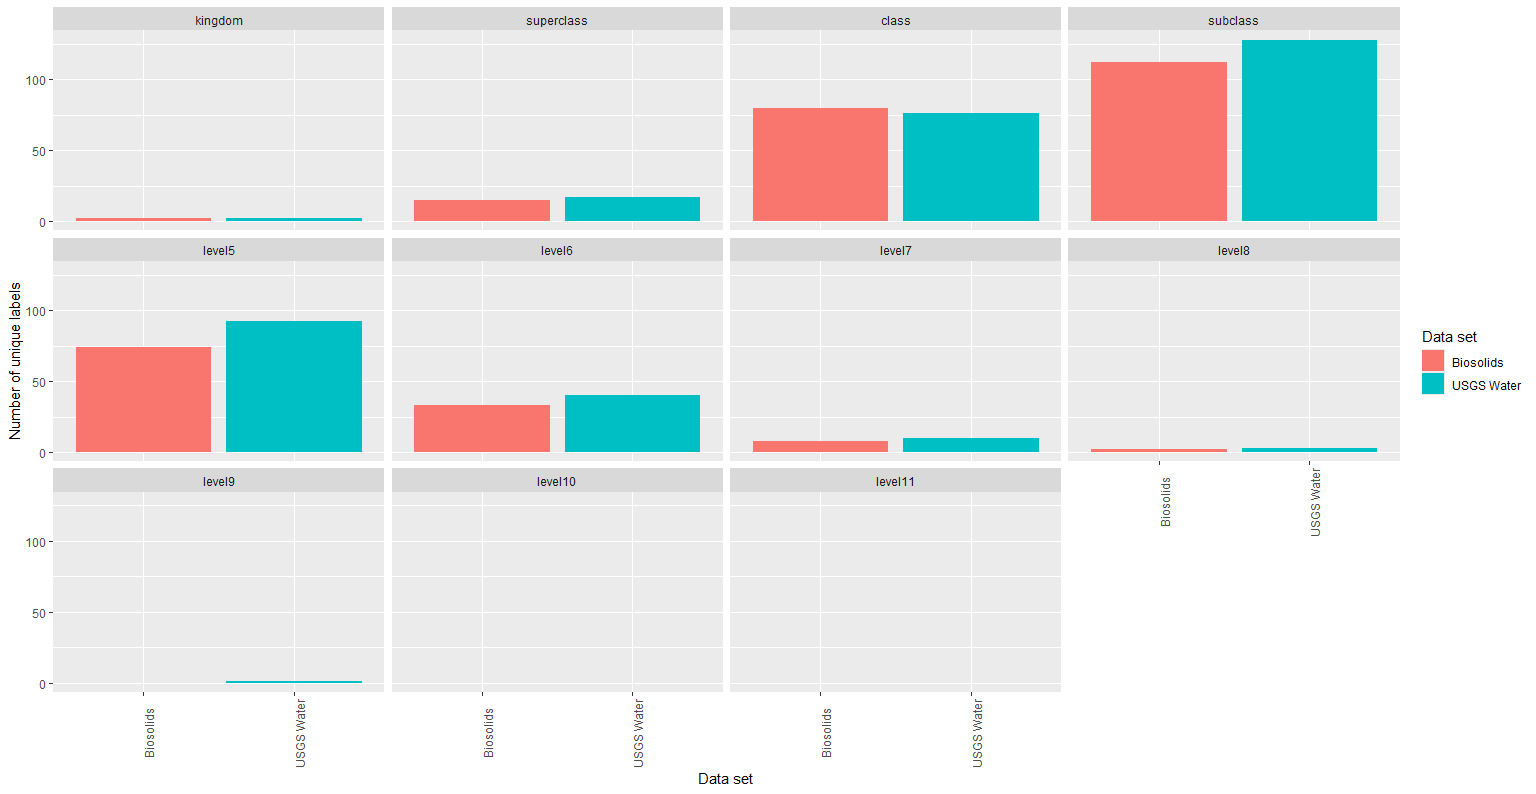
\includegraphics{label-bars_2}
\caption{\label{fig:lab-bars-2} This figure displays the counts of unique labels broken down by dataset and faceted by each classification level.}
\end{figure}

From Figure \ref{fig:label-bars_1} and Figure \ref{fig:label-bars_2}, we see that the distribution of numbers of labels across taxonomic levels is relatively similar for each data set, though in general the \code{usgswater\_classified} data has more labels than the \code{biosolids\_classified} data at each level. However, this does not give us a sense of how these labels spread through chemical space as defined by ChemOnt nor does it characterize the overlap between the classifications of these data sets. To investigate these aspects of chemical space coverage further, we use tree-based visualizations.

\section{Tree visualizations} \label{sec:trees}

The tree visualizations developed in \pkg{treecompareR} rely heavily on the \pkg{ggtree} package, which was designed with visualization of phylogenetic trees in mind. The \pkg{ggtree} package extends the widely used \pkg{ggplot2} package, greatly broadening the variety and scope of tree visualizations available for use.

We first display the ChemOnt tree, the taxonomy structure of the ChemOnt ontology, in a circular layout format.

%
\begin{Schunk}
\begin{Sinput}
R> ggtree(chemont_tree) + layout_circular()
\end{Sinput}
\end{Schunk}
%

\begin{figure}[t!]
\centering
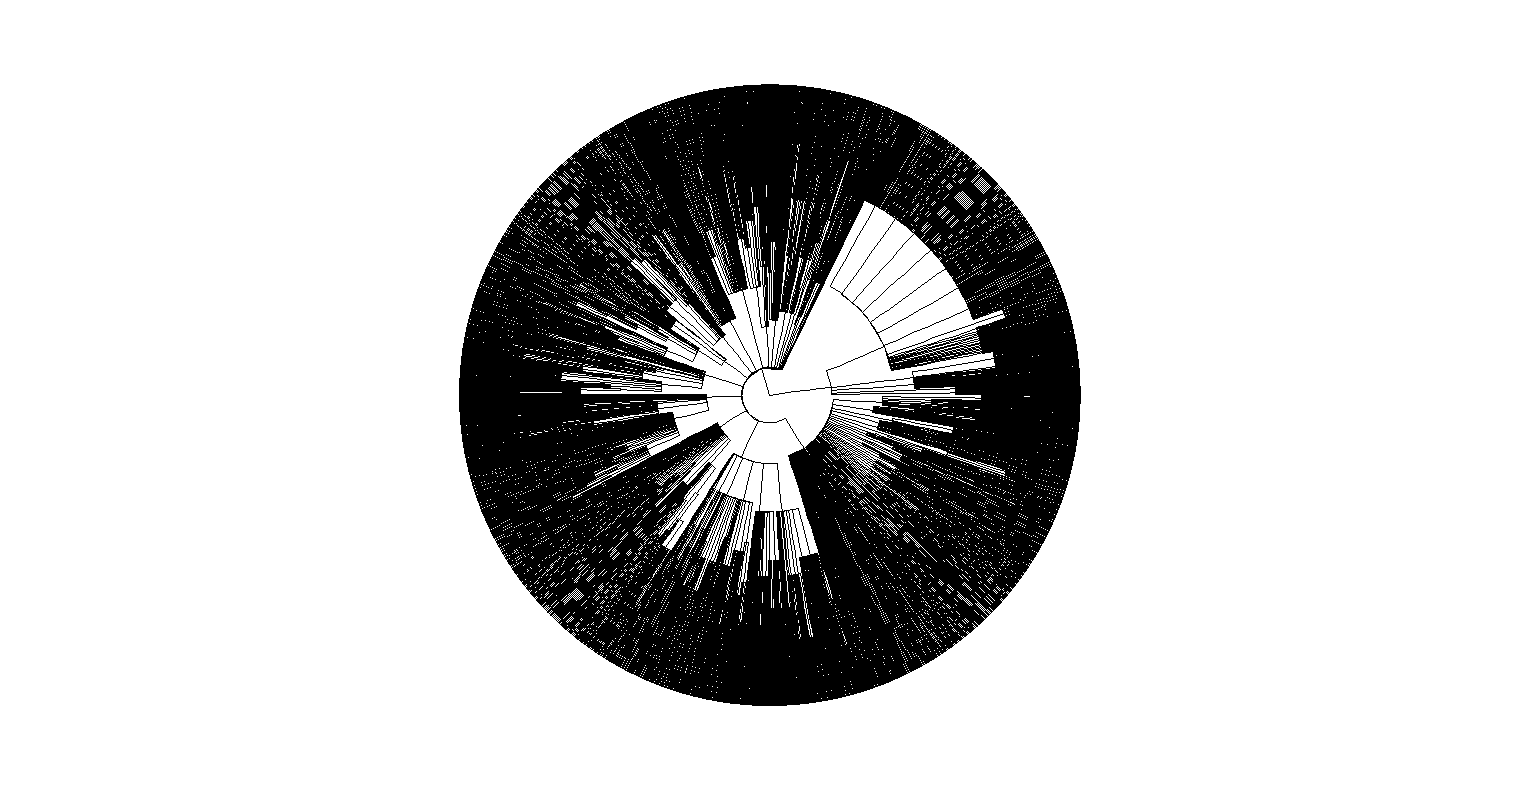
\includegraphics{chemont-tree}
\caption{\label{fig:chemont-tree} The Chemont tree displayed in a circular layout.}
\end{figure}

The diagram \ref{fig:chemont-tree} illustrates the scope of the taxonomy structure of the ChemOnt ontology. From this diagram we create visualizations that highlight the areas of chemical space each data set represents. This ChemOnt tree diagram displays a tree with 3612 tips and 1213 internal nodes (including the root of the tree). As one can easily observe, this creates a dense tree visualization that requires additional attention to be of greater use.

We first examine which parts of this tree are given by classifications of chemicals in each data set. To do this, we use the function \fct{display\_subtree}. This function takes in a \pkg{data.table} with classification data and returns a tree diagram highlighting membership for each node and tip of the full ChemOnt tree. Branches and nodes in the tree are highlighted different colors depending on whether they are included in the set of classification labels of the \pkg{data.table}. In this example we also display the tip labels.

%
\begin{Schunk}
\begin{Sinput}
R> display_subtree(data_1 = biosolids_classified,
+                  name_1 = 'Biosolids')
\end{Sinput}
\end{Schunk}
%

\begin{figure}[t!]
\centering
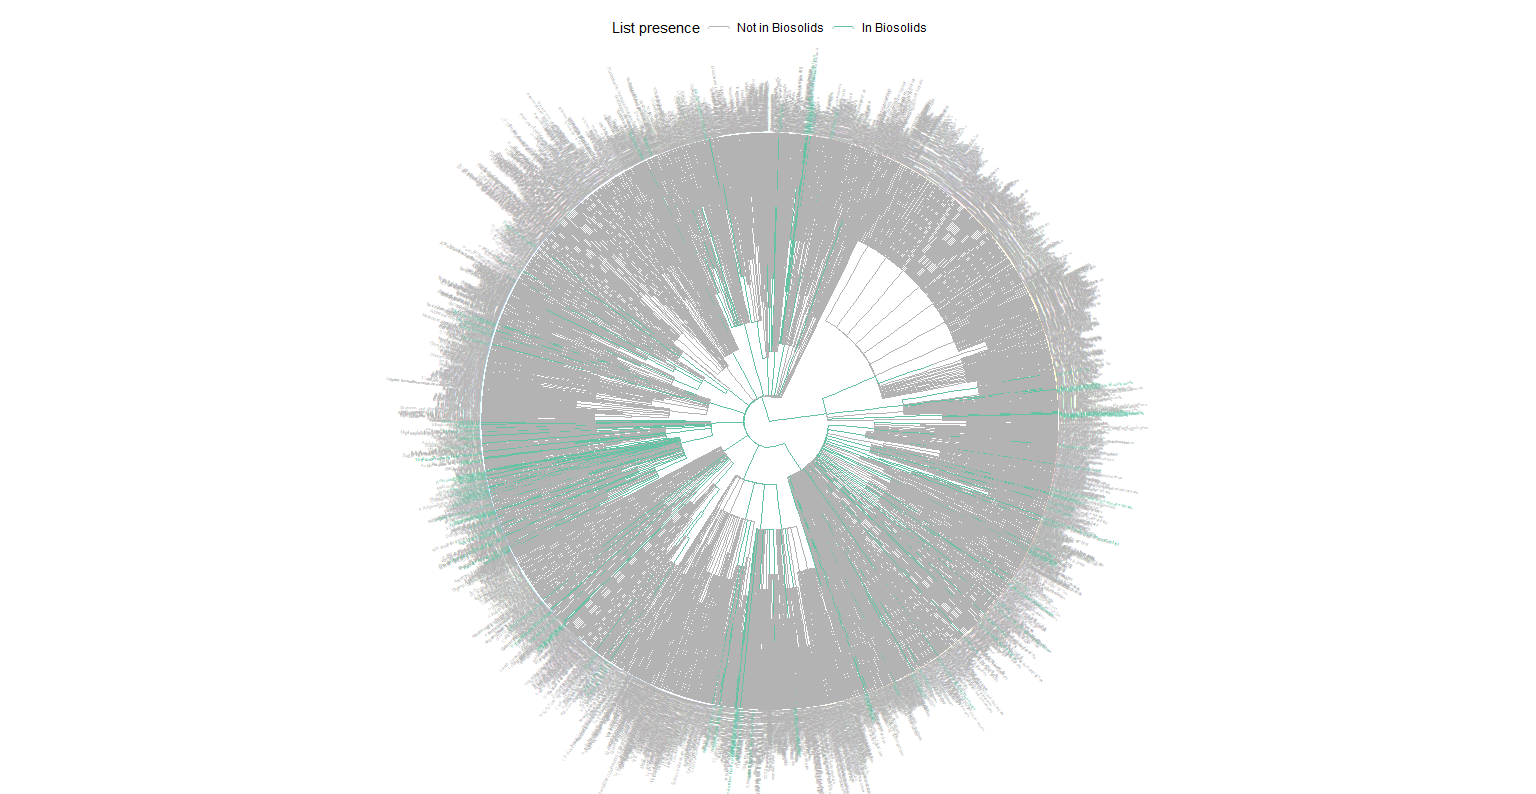
\includegraphics{biosolids-subtree}
\caption{\label{fig:biosolids-subtree} The Biosolids subtree displayed within the full Chemont tree, with tip labels included.}
\end{figure}

%
\begin{Schunk}
\begin{Sinput}
R> display_subtree(data_1 = biosolids_classified,
+                  name_1 = 'Biosolids')
\end{Sinput}
\end{Schunk}
%

\begin{figure}[t!]
\centering
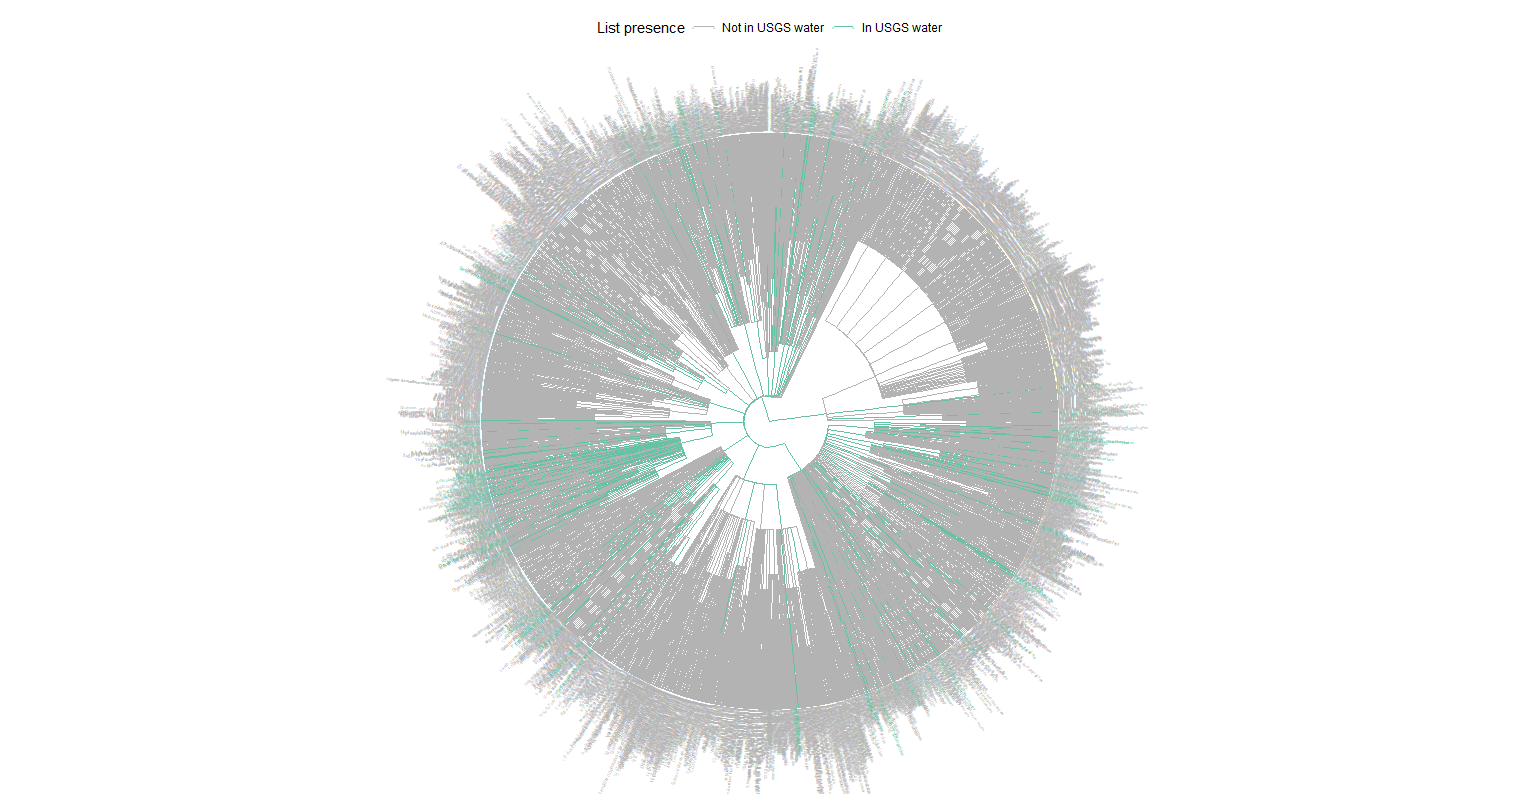
\includegraphics{usgs-water-subtree}
\caption{\label{fig:usgs-water-tree} The USGS Water subtree displayed within the full Chemont tree, with tip labels included.}
\end{figure}


In the Figure \ref{fig:biosolids-subtree} and Figure \ref{fig:usgs-water-tree}, we observe that the labels and branches represented by classifications from each data set are shaded green while labels and branches not present in the classifications are shaded grey. This helps illustrate where in chemical space these classification labels are located. While it is possible to compare each diagram individually to get a sense of how each data set represents chemical space, it would be better if we could directly compare the subtrees they represent. We can do just that using the exact same function, inputting both data sets into the function \fct{display\_subtree} as the following example demonstrates.

%
\begin{Schunk}
\begin{Sinput}
R> display_subtree(data_1 = biosolids_classified,
+                  data_2 = usgswater_classified,
+                  name_1 = 'Biosolids',
+                  name_2 = 'USGS Water')
\end{Sinput}
\end{Schunk}
%

\begin{figure}[t!]
\centering
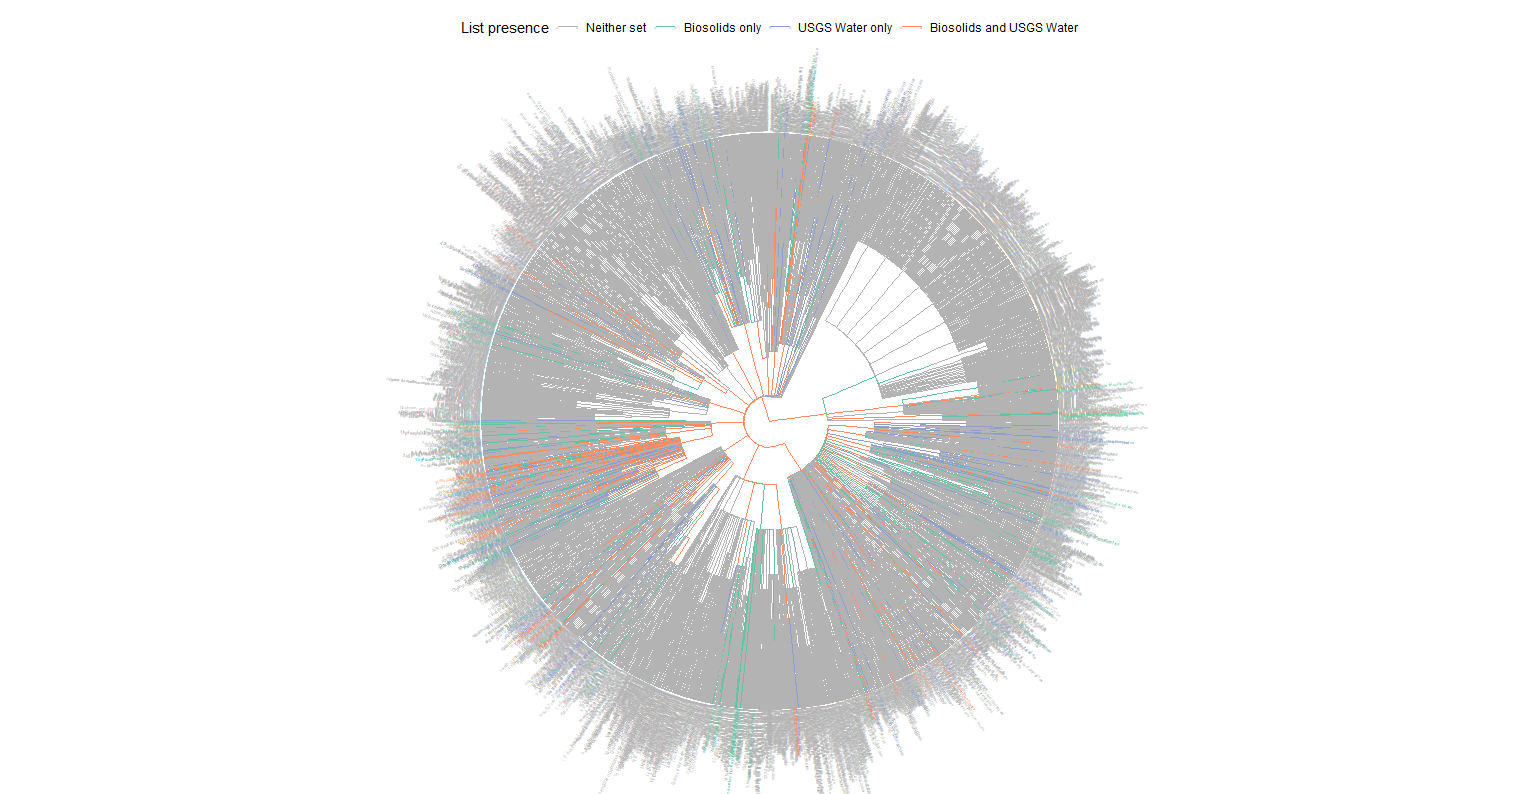
\includegraphics{subtree-overlap}
\caption{\label{fig:subtree-overlap} The Biosolids and USGS Water subtrees displayed together within the full Chemont tree, with tip labels included. Classification labels are colored based on whether they are represented by either data set, both, or neither.}
\end{figure}

In Figure \ref{fig:subtree-overlap}, branches and labels are colored based on whether they are members of classifications of one, both, or neither data set. This gives an indication of how the chemical space represented by each data set overlaps through visualization of the induced subtrees within the full ChemOnt tree. From this visualization, it is also possible to determine the areas in chemical space unique to each data set.

While this particular visual can be informative, if the taxonomy is fairly large compared to the subtree induced by a data set, the diagram generated by \fct{display\_subtree} can be cluttered and difficult to interpret. One solution for improving clarity is by pruning away extraneous branches and labels not represented by the subtree. We demonstrate this using the function \fct{prune\_and\_display\_subtree} on both data sets.

%
\begin{Schunk}
\begin{Sinput}
R> prune_and_display_subtree(prune_to = biosolids_classified)
R> prune_and_display_subtree(prune_to = usgswater_classified)
\end{Sinput}
\end{Schunk}
%

\begin{figure}[t!]
\centering
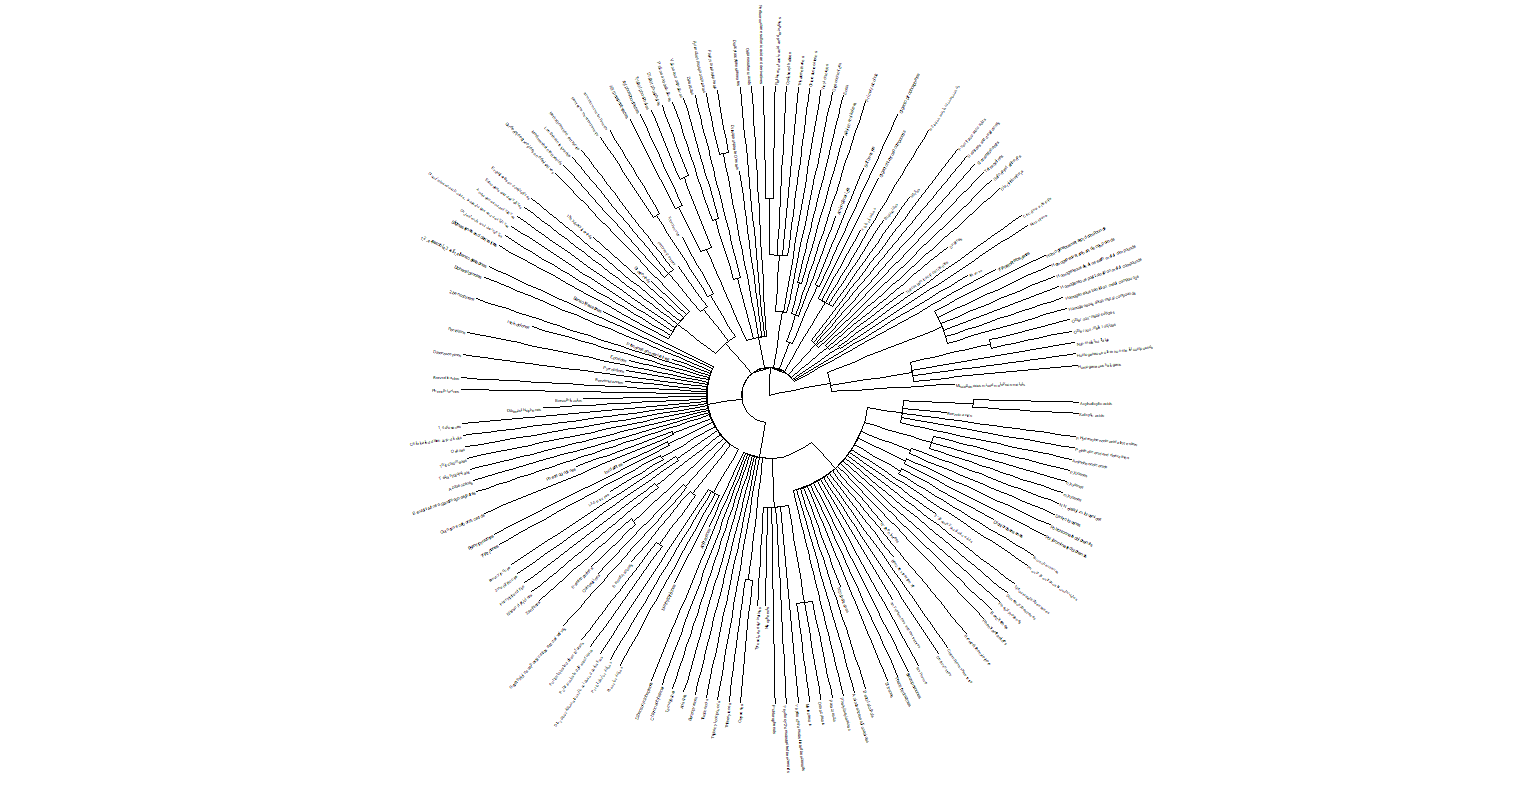
\includegraphics{biosolids-prune-subtree}
\caption{\label{fig:prune-biosolids} The biosolids subtree pruned from the Chemont tree.}
\end{figure}


\begin{figure}[t!]
\centering
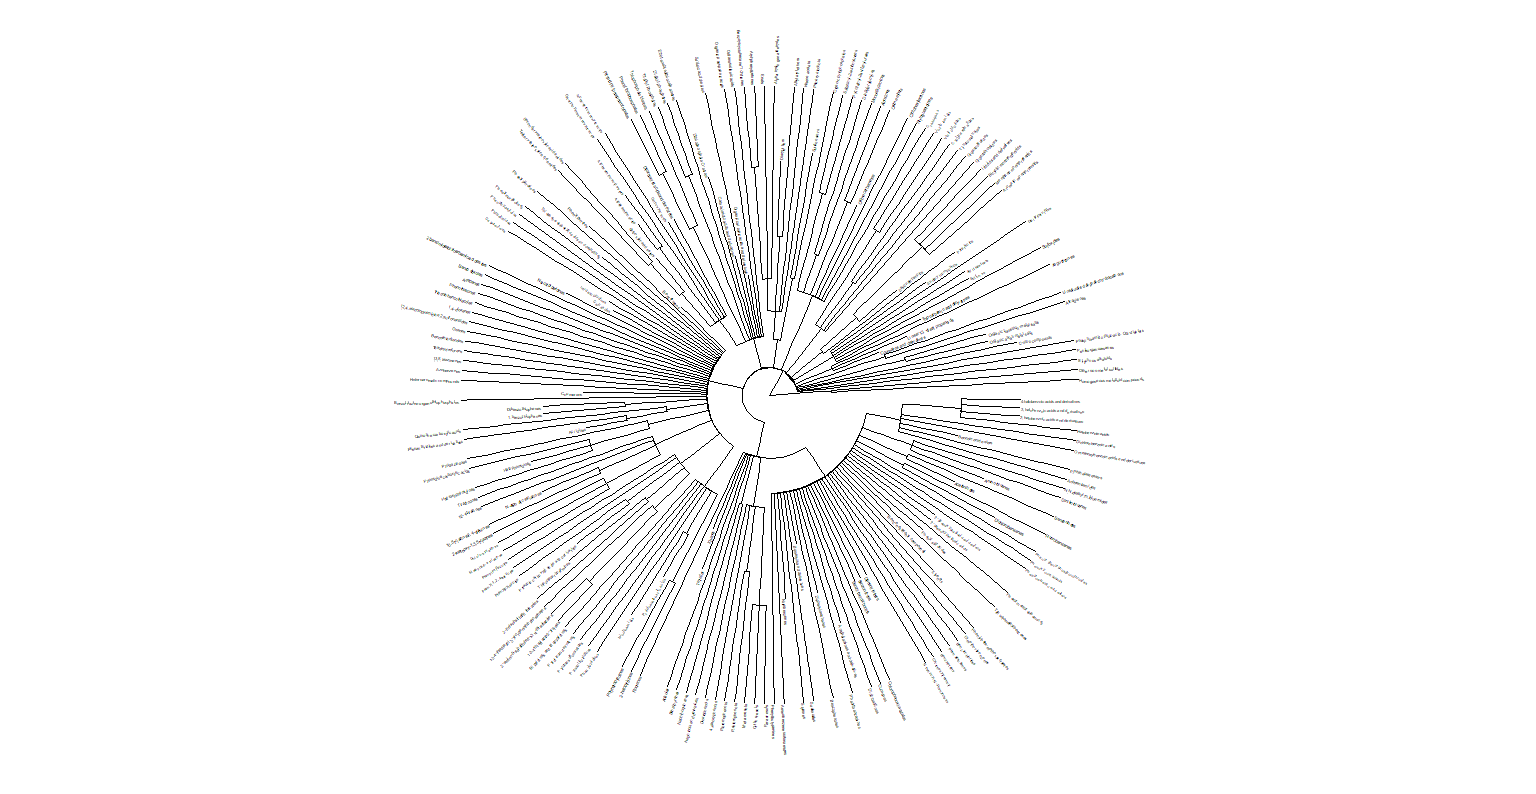
\includegraphics{usgswater-prune-subtree}
\caption{\label{fig:prune-usgswater} The usgswater subtree pruned from the Chemont tree.}
\end{figure}

In Figure \ref{fig:prune-biosolids} and Figure \ref{fig:prune-usgswater}, the extraneous branches and tips not included in the set of classification labels of the data set are pruned and the remaining subtree is displayed. While there is still a lot of information displayed through the tip labels, this visualization provides a much closer look at the subtree induced by the data set than the previous visual that displayed the subtree within the whole taxonomy. Also observe that the shape of the subtree, while similar to the shape of the subtree displayed within the full ChemOnt tree, may change based on the set of extraneous branches and nodes that are pruned away.

We note a few things about this diagram and the \fct{prune\_and\_display\_subtree} function. First, the output of the function is a diagram of the subtree (or just the \code{phylo} object if the function parameter \code{no\_plot = TRUE} is used). Second, while many chemical classifications terminate with a tip label as the most specific label in the classification, there are some classifications that terminate with an internal node. If we were just to delete the internal nodes and tips not represented by classifications for a data set using \fct{ape::drop.tip}, the internal nodes that were terminal labels (and now are tips of the subtree) for classifications would appear in the diagram somewhere between the outer layer of tips and the root. The \fct{prune\_and\_display\_subtree} function adjusts the branch lengths to accommodate the new structure of the subtree and extends these newly created tip labels of the subtree to match the pre-existing tip labels. This is recorded in the \code{edge.length} list of the output \code{phylo} object. A visual comparison between the branches in the subtree and the subtree within the entire taxonomy may show slight differences as a result of this branch adjustment. Third, with the omission of the extraneous branches and labels, there is the possibility that branches of the pruned subtree have rotate relative to their orientation within the ChemOnt tree. The structure of the subtree is the same, but the visual representation may differ.

In a manner similar to the output of \fct{display\_subtree} when comparing two data sets, we may wish to look at the induced subtrees of two different data sets and compare membership of labels in one subtree with the other subtree. To achieve this, we use the function \fct{data\_set\_subtrees} as we illustrate in the following example.

%
\begin{Schunk}
\begin{Sinput}
R> data_set_subtrees(data_1 = biosolids_classified,
+                    data_2 = usgswater_classified,
+                    name_1 = 'Biosolids',
+                    name_2 = 'USGS water')
\end{Sinput}
\end{Schunk}
%






%% -- Manuscript ---------------------------------------------------------------

%% - In principle "as usual" again.
%% - When using equations (e.g., {equation}, {eqnarray}, {align}, etc.
%%   avoid empty lines before and after the equation (which would signal a new
%%   paragraph.
%% - When describing longer chunks of code that are _not_ meant for execution
%%   (e.g., a function synopsis or list of arguments), the environment {Code}
%%   is recommended. Alternatively, a plain {verbatim} can also be used.
%%   (For executed code see the next section.)

\section{Models and software} \label{sec:models}

The basic Poisson regression model for count data is a special case of the GLM
framework \cite{McCullagh+Nelder:1989}. It describes the dependence of a count
response variable $y_i$ ($i = 1, \dots, n$) by assuming a Poisson distribution
$y_i \sim \mathrm{Pois}(\mu_i)$. The dependence of the conditional mean
$\E[y_i \, | \, x_i] = \mu_i$ on the regressors $x_i$ is then specified via a
log link and a linear predictor
%
\begin{equation} \label{eq:mean}
\log(\mu_i) \quad = \quad x_i^\top \beta,
\end{equation}
%
where the regression coefficients $\beta$ are estimated by maximum likelihood
(ML) using the iterative weighted least squares (IWLS) algorithm.

\begin{leftbar}
Note that around the \verb|{equation}| above there should be no spaces (avoided
in the {\LaTeX} code by \verb|%| lines) so that ``normal'' spacing is used and
not a new paragraph started.
\end{leftbar}

\proglang{R} provides a very flexible implementation of the general GLM
framework in the function \fct{glm} \citep{Chambers+Hastie:1992} in the
\pkg{stats} package. Its most important arguments are
\begin{Code}
glm(formula, data, subset, na.action, weights, offset,
  family = gaussian, start = NULL, control = glm.control(...),
  model = TRUE, y = TRUE, x = FALSE, ...)
\end{Code}
where \code{formula} plus \code{data} is the now standard way of specifying
regression relationships in \proglang{R}/\proglang{S} introduced in
\cite{Chambers+Hastie:1992}. The remaining arguments in the first line
(\code{subset}, \code{na.action}, \code{weights}, and \code{offset}) are also
standard  for setting up formula-based regression models in
\proglang{R}/\proglang{S}. The arguments in the second line control aspects
specific to GLMs while the arguments in the last line specify which components
are returned in the fitted model object (of class \class{glm} which inherits
from \class{lm}). For further arguments to \fct{glm} (including alternative
specifications of starting values) see \code{?glm}. For estimating a Poisson
model \code{family = poisson} has to be specified.

\begin{leftbar}
As the synopsis above is a code listing that is not meant to be executed,
one can use either the dedicated \verb|{Code}| environment or a simple
\verb|{verbatim}| environment for this. Again, spaces before and after should be
avoided.

Finally, there might be a reference to a \verb|{table}| such as
Table~\ref{tab:overview}. Usually, these are placed at the top of the page
(\verb|[t!]|), centered (\verb|\centering|), with a caption below the table,
column headers and captions in sentence style, and if possible avoiding vertical
lines.
\end{leftbar}

\begin{table}[t!]
\centering
\begin{tabular}{lllp{7.4cm}}
\hline
Type           & Distribution & Method   & Description \\ \hline
GLM            & Poisson      & ML       & Poisson regression: classical GLM,
                                           estimated by maximum likelihood (ML) \\
               &              & Quasi    & ``Quasi-Poisson regression'':
                                           same mean function, estimated by
                                           quasi-ML (QML) or equivalently
                                           generalized estimating equations (GEE),
                                           inference adjustment via estimated
                                           dispersion parameter \\
               &              & Adjusted & ``Adjusted Poisson regression'':
                                           same mean function, estimated by
                                           QML/GEE, inference adjustment via
                                           sandwich covariances\\
               & NB           & ML       & NB regression: extended GLM,
                                           estimated by ML including additional
                                           shape parameter \\ \hline
Zero-augmented & Poisson      & ML       & Zero-inflated Poisson (ZIP),
                                           hurdle Poisson \\
               & NB           & ML       & Zero-inflated NB (ZINB),
                                           hurdle NB \\ \hline
\end{tabular}
\caption{\label{tab:overview} Overview of various count regression models. The
table is usually placed at the top of the page (\texttt{[t!]}), centered
(\texttt{centering}), has a caption below the table, column headers and captions
are in sentence style, and if possible vertical lines should be avoided.}
\end{table}


%% -- Illustrations ------------------------------------------------------------

%% - Virtually all JSS manuscripts list source code along with the generated
%%   output. The style files provide dedicated environments for this.
%% - In R, the environments {Sinput} and {Soutput} - as produced by Sweave() or
%%   or knitr using the render_sweave() hook - are used (without the need to
%%   load Sweave.sty).
%% - Equivalently, {CodeInput} and {CodeOutput} can be used.
%% - The code input should use "the usual" command prompt in the respective
%%   software system.
%% - For R code, the prompt "R> " should be used with "+  " as the
%%   continuation prompt.
%% - Comments within the code chunks should be avoided - these should be made
%%   within the regular LaTeX text.

\section{Illustrations} \label{sec:illustrations}

For a simple illustration of basic Poisson and NB count regression the
\code{quine} data from the \pkg{MASS} package is used. This provides the number
of \code{Days} that children were absent from school in Australia in a
particular year, along with several covariates that can be employed as regressors.
The data can be loaded by
%
\begin{Schunk}
\begin{Sinput}
R> data("quine", package = "MASS")
\end{Sinput}
\end{Schunk}
%
and a basic frequency distribution of the response variable is displayed in
Figure~\ref{fig:quine}.

\begin{leftbar}
For code input and output, the style files provide dedicated environments.
Either the ``agnostic'' \verb|{CodeInput}| and \verb|{CodeOutput}| can be used
or, equivalently, the environments \verb|{Sinput}| and \verb|{Soutput}| as
produced by \fct{Sweave} or \pkg{knitr} when using the \code{render_sweave()}
hook. Please make sure that all code is properly spaced, e.g., using
\code{y = a + b * x} and \emph{not} \code{y=a+b*x}. Moreover, code input should
use ``the usual'' command prompt in the respective software system. For
\proglang{R} code, the prompt \code{"R> "} should be used with \code{"+  "} as
the continuation prompt. Generally, comments within the code chunks should be
avoided -- and made in the regular {\LaTeX} text instead. Finally, empty lines
before and after code input/output should be avoided (see above).
\end{leftbar}

\begin{figure}[t!]
\centering
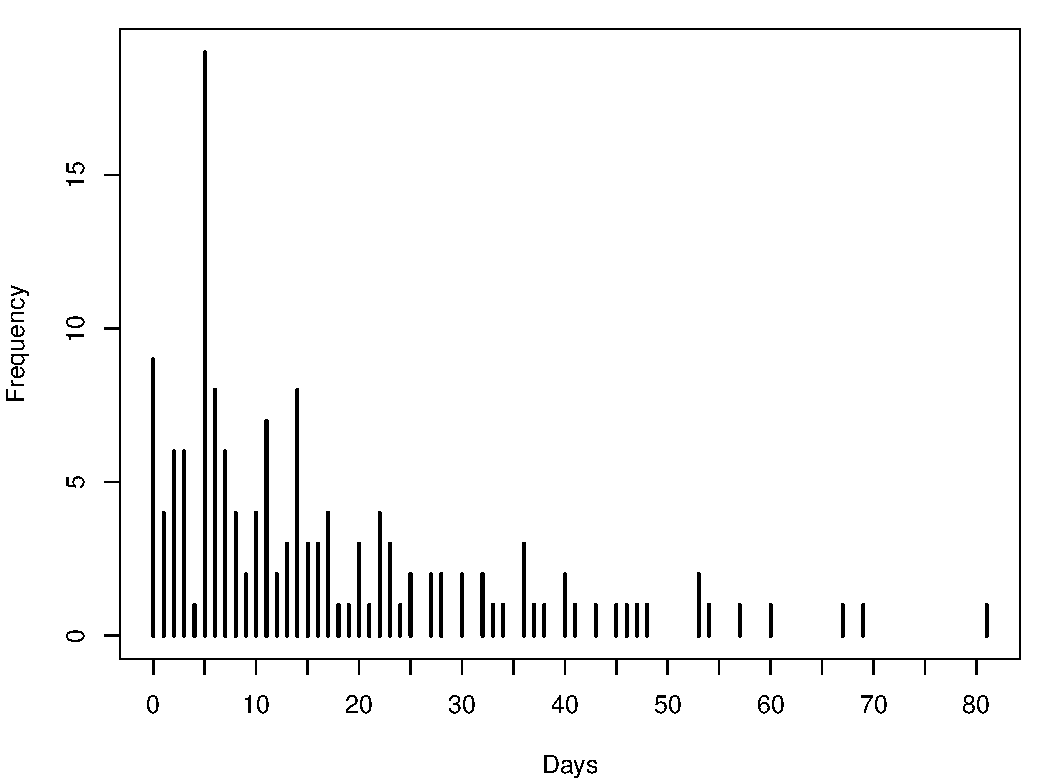
\includegraphics{treecompareR_JSS_ms-visualization}
\caption{\label{fig:quine} Frequency distribution for number of days absent
from school.}
\end{figure}

As a first model for the \code{quine} data, we fit the basic Poisson regression
model. (Note that JSS prefers when the second line of code is indented by two
spaces.)
%
\begin{Schunk}
\begin{Sinput}
R> m_pois <- glm(Days ~ (Eth + Sex + Age + Lrn)^2, data = quine,
+    family = poisson)
\end{Sinput}
\end{Schunk}
%
To account for potential overdispersion we also consider a negative binomial
GLM.
%
\begin{Schunk}
\begin{Sinput}
R> library("MASS")
R> m_nbin <- glm.nb(Days ~ (Eth + Sex + Age + Lrn)^2, data = quine)
\end{Sinput}
\end{Schunk}
%
In a comparison with the BIC the latter model is clearly preferred.
%
\begin{Schunk}
\begin{Sinput}
R> BIC(m_pois, m_nbin)
\end{Sinput}
\begin{Soutput}
       df      BIC
m_pois 18 2046.851
m_nbin 19 1157.235
\end{Soutput}
\end{Schunk}
%
Hence, the full summary of that model is shown below.
%
\begin{Schunk}
\begin{Sinput}
R> summary(m_nbin)
\end{Sinput}
\begin{Soutput}
Call:
glm.nb(formula = Days ~ (Eth + Sex + Age + Lrn)^2, data = quine, 
    init.theta = 1.60364105, link = log)

Coefficients: (1 not defined because of singularities)
            Estimate Std. Error z value Pr(>|z|)    
(Intercept)  3.00155    0.33709   8.904  < 2e-16 ***
EthN        -0.24591    0.39135  -0.628  0.52977    
SexM        -0.77181    0.38021  -2.030  0.04236 *  
AgeF1       -0.02546    0.41615  -0.061  0.95121    
AgeF2       -0.54884    0.54393  -1.009  0.31296    
AgeF3       -0.25735    0.40558  -0.635  0.52574    
LrnSL        0.38919    0.48421   0.804  0.42153    
EthN:SexM    0.36240    0.29430   1.231  0.21818    
EthN:AgeF1  -0.70000    0.43646  -1.604  0.10876    
EthN:AgeF2  -1.23283    0.42962  -2.870  0.00411 ** 
EthN:AgeF3   0.04721    0.44883   0.105  0.91622    
EthN:LrnSL   0.06847    0.34040   0.201  0.84059    
SexM:AgeF1   0.02257    0.47360   0.048  0.96198    
SexM:AgeF2   1.55330    0.51325   3.026  0.00247 ** 
SexM:AgeF3   1.25227    0.45539   2.750  0.00596 ** 
SexM:LrnSL   0.07187    0.40805   0.176  0.86019    
AgeF1:LrnSL -0.43101    0.47948  -0.899  0.36870    
AgeF2:LrnSL  0.52074    0.48567   1.072  0.28363    
AgeF3:LrnSL       NA         NA      NA       NA    
---
Signif. codes:  0 '***' 0.001 '**' 0.01 '*' 0.05 '.' 0.1 ' ' 1

(Dispersion parameter for Negative Binomial(1.6036) family taken to be 1)

    Null deviance: 235.23  on 145  degrees of freedom
Residual deviance: 167.53  on 128  degrees of freedom
AIC: 1100.5

Number of Fisher Scoring iterations: 1


              Theta:  1.604 
          Std. Err.:  0.214 

 2 x log-likelihood:  -1062.546 
\end{Soutput}
\end{Schunk}



%% -- Summary/conclusions/discussion -------------------------------------------

\section{Summary and discussion} \label{sec:summary}

\begin{leftbar}
As usual \dots
\end{leftbar}


%% -- Optional special unnumbered sections -------------------------------------

\section*{Computational details}

\begin{leftbar}
If necessary or useful, information about certain computational details
such as version numbers, operating systems, or compilers could be included
in an unnumbered section. Also, auxiliary packages (say, for visualizations,
maps, tables, \dots) that are not cited in the main text can be credited here.
\end{leftbar}

The results in this paper were obtained using
\proglang{R}~.4 with the
\pkg{MASS}~7.3.61 package. \proglang{R} itself
and all packages used are available from the Comprehensive
\proglang{R} Archive Network (CRAN) at
\url{https://CRAN.R-project.org/}.


\section*{Acknowledgments}

\begin{leftbar}
All acknowledgments (note the AE spelling) should be collected in this
unnumbered section before the references. It may contain the usual information
about funding and feedback from colleagues/reviewers/etc. Furthermore,
information such as relative contributions of the authors may be added here
(if any).
\end{leftbar}


%% -- Bibliography -------------------------------------------------------------
%% - References need to be provided in a .bib BibTeX database.
%% - All references should be made with \cite, \citet, \citep, \citealp etc.
%%   (and never hard-coded). See the FAQ for details.
%% - JSS-specific markup (\proglang, \pkg, \code) should be used in the .bib.
%% - Titles in the .bib should be in title case.
%% - DOIs should be included where available.

\bibliography{refs}


%% -- Appendix (if any) --------------------------------------------------------
%% - After the bibliography with page break.
%% - With proper section titles and _not_ just "Appendix".

\newpage

\begin{appendix}

\section{More technical details} \label{app:technical}

\begin{leftbar}
Appendices can be included after the bibliography (with a page break). Each
section within the appendix should have a proper section title (rather than
just \emph{Appendix}).

For more technical style details, please check out JSS's style FAQ at
\url{https://www.jstatsoft.org/pages/view/style#frequently-asked-questions}
which includes the following topics:
\begin{itemize}
  \item Title vs.\ sentence case.
  \item Graphics formatting.
  \item Naming conventions.
  \item Turning JSS manuscripts into \proglang{R} package vignettes.
  \item Trouble shooting.
  \item Many other potentially helpful details\dots
\end{itemize}
\end{leftbar}


\section[Using BibTeX]{Using \textsc{Bib}{\TeX}} \label{app:bibtex}

\begin{leftbar}
References need to be provided in a \textsc{Bib}{\TeX} file (\code{.bib}). All
references should be made with \verb|\cite|, \verb|\citet|, \verb|\citep|,
\verb|\citealp| etc.\ (and never hard-coded). This commands yield different
formats of author-year citations and allow to include additional details (e.g.,
pages, chapters, \dots) in brackets. In case you are not familiar with these
commands see the JSS style FAQ for details.

Cleaning up \textsc{Bib}{\TeX} files is a somewhat tedious task -- especially
when acquiring the entries automatically from mixed online sources. However,
it is important that informations are complete and presented in a consistent
style to avoid confusions. JSS requires the following format.
\begin{itemize}
  \item JSS-specific markup (\verb|\proglang|, \verb|\pkg|, \verb|\code|) should
    be used in the references.
  \item Titles should be in title case.
  \item Journal titles should not be abbreviated and in title case.
  \item DOIs should be included where available.
  \item Software should be properly cited as well. For \proglang{R} packages
    \code{citation("pkgname")} typically provides a good starting point.
\end{itemize}
\end{leftbar}

\end{appendix}

%% -----------------------------------------------------------------------------


\end{document}
